\documentclass[12pt, letterpaper]{article}

\usepackage{graphicx}
\usepackage{amsmath}

\title{Optical Pumping}
\author{Jay Shen}
\date{February 2025}

\begin{document}

\maketitle

Optical pumping is a method to excite atoms into certain energy states using light. In this paper, we make use of an optical pumping setup to study the weak and strong field Zeeman effects in a Rubidium gas. 

\section{Calibration} \label{sec:calibration}

As will become evident in Sections \ref{sec:weak} and \ref{sec:strong}, our experiment relies on knowing the current passing through the horizontal field sweep coil. To determine this current, we measure the voltage produced by the sweep function generator. However, since the oscilloscope we use may be off by a constant of proportionality, we must determine a suitable calibration function to map the oscilloscope voltage reading to the true current passing through the coil. 

To accomplish this, we took measurements of the oscilloscope voltage reading for various sweep settings, and simultaneously read the current passing through the coil using a multimeter. These figures are listed in Table \ref{tab:calibration}. 

\begin{table}[!h]
    \centering
    \begin{tabular}{| c | c |}
        \hline
        $I_M$ (amps) &  $V_S$ (volts) \\
        \hline
        $0.0962 \pm 0.0001$ & $-13.40 \pm 0.10$ \\
        $0.1279 \pm 0.0001$ & $-12.50 \pm 0.10$ \\
        $0.1918 \pm 0.0001$ & $-10.60 \pm 0.10$ \\
        $0.2894 \pm 0.0001$ & $-7.60 \pm 0.10$ \\
        $0.4060 \pm 0.0010$ & $-4.00 \pm 0.10$ \\
        $0.5040 \pm 0.0010$ & $-1.00 \pm 0.10$ \\
        $0.6060 \pm 0.0010$ & $2.03 \pm 0.01$ \\
        $0.6860 \pm 0.0010$ & $4.59 \pm 0.01$ \\
        $0.7860 \pm 0.0010$ & $7.59 \pm 0.01$ \\
        $0.8800 \pm 0.0010$ & $10.40 \pm 0.01$ \\
        $0.9780 \pm 0.0010$ & $13.30 \pm 0.01$ \\
        \hline
    \end{tabular}
    \caption{Measurements of current $I$ measured by multimeter and oscilloscope voltage $V_S$}
    \label{tab:calibration}
\end{table}

Visual inspection immediately tells us that this data is linear, so we fit a function $I = a V_S + b$ as shown in Figure \ref{fig:calibration}. 
\begin{figure}[!h]
    \centering
    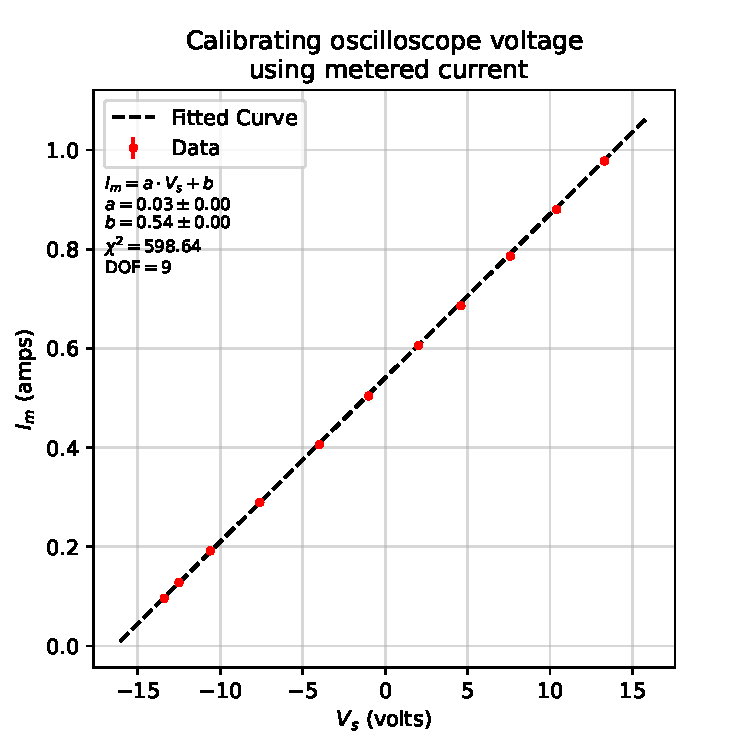
\includegraphics[width=0.75\textwidth]{experiment4/figures/calibration.pdf}
    \caption{}
    \label{fig:calibration}
\end{figure}
The fit we achieve is very good, and the linear curve visually models the data almost perfectly. We determine that $a = 0.033033 \pm 0.000016$ and $b = 0.54046 \pm 0.00018$, which have fairly low uncertainties. Our reduced chi-square score $\bar{\chi}^2 = 66.52$ is somewhat high, however we attribute this to the small sample size. 

\section{The weak field Zeeman effect} \label{sec:weak}

We now move to observe the weak field Zeeman effect for rubidium gas. Our setup uses RF depumping to drive electronic transitions between Zeeman states. Namely, we use an oscillating electromagnetic field (EMF) to bombard the rubidium with photons. When the photon energy matches the energy difference between Zeeman states, transitions are driven amongst the rubidium atoms and they are temporarily depumped. These depumped atoms absorb light and we observe a dip in the PMT signal. Figure \ref{fig:weak-scope} shows this phenomena as measured by an oscilloscope. 

\begin{figure}[!h]
    \centering
    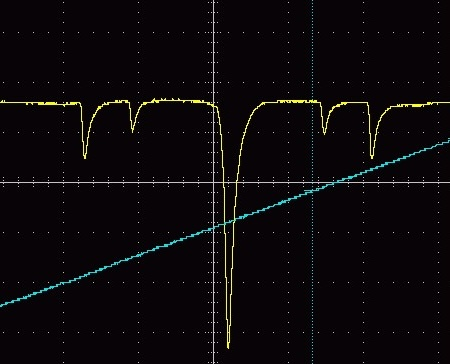
\includegraphics[width=0.75\textwidth]{experiment4/figures/weak.jpg}
    \caption{An oscilloscope screenshot showing RF depumping dips. The yellow line is the PMT reading and the blue line is the horizontal sweep voltage. From left to right, the peaks represent Rb-87 depumping, Rb-85 depumping, zero-field depumping, Rb-85 depumping, and Rb-87 depumping. }
    \label{fig:weak-scope}
\end{figure}

\subsection{Theory of Zeeman splitting and RF depumping}

We can model these dips using the theory of Zeeman splitting. The energy difference between Zeeman states is
\begin{equation}\label{eq:zeeman}
    \Delta E = \mu_B g_f \Delta m_f B \approx \mu_B g_f B
\end{equation}
where $\mu_B$ is a known constant. When an atom transitions between Zeeman states and depumps, the energy provided by the photon must be $E_p = \Delta E$. For an EMF oscillating with frequency $f$, we know the energy of its photons is $E_p = hf$. So at each depumping dip, $\Delta E = E_p = hf$

We also known the value of $B$ at any given time to be
\begin{equation}\label{eq:helmholtz}
    B = \Bigr(\:\frac{4}{5} \: \Bigr )^{3/2} \frac{\mu_0 n I}{R}
\end{equation}
Here, $\mu_0$, $n$, and $R$ are known constants, and $I$ is the current passing through the horizontal sweep coil. 

\subsection{Measurements}

We seek to evaluate this theory empirically by collecting values of $\Delta E$ and $B$ in order to fit a value for $g_f$. 

Setting values of $\Delta E$ is straightforward as we have fine-grain control over the RF frequency $f$. To measure $B$, we compute it from $I$ using Equation \ref{eq:helmholtz}. We get $I$ from $V_S$ using our calibration equation $I = a V_S + b$ from Section \ref{sec:calibration}. At time of depumping, $V_S$ is the voltage over the horizontal sweep. To remove the oscilloscope phase, we measure $V_S$ as the voltage difference from the zero-field peak, where the voltage is known to be zero. Figure \ref{fig:weak-measurement} shows this measurement visually. 

\begin{figure}[!h]
    \centering
    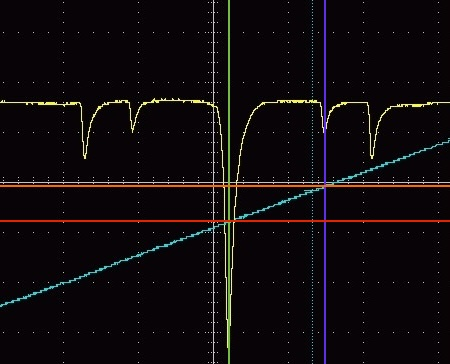
\includegraphics[width=0.75\textwidth]{experiment4/figures/weak_measurement.jpg}
    \caption{The horizontal sweep voltage $V_S$ is measured as the voltage difference from the zero-field dip. The green and purple vertical cursors indicate the time of zero-field and a Rb-85 depumping dip, respectively. The red and orange horizontal cursors indicate the oscilloscope voltage at those times. $V_S$ is then the difference in readings between the red and orange cursors. }
    \label{fig:weak-measurement}
\end{figure}

Following this procedure, we varied $f$ and measured $V_S$ for two dips corresponding to Rb-85 and Rb-87 depumping. These measurements are recorded in Table \ref{tab:weak}. 

\begin{table}[!h]
    \centering
    \begin{tabular}{| c | c | c |}
        \hline
        & Rb-87  & Rb-85 \\
        \hline
        $f$ (Hz) &  $V_S$ (volts) & $V_S$ (volts) \\
        \hline
        $20000 \pm 1$ & $1.4 \pm 0.1$ & $2.0 \pm 0.1$ \\
        $30000 \pm 1$ & $2.0 \pm 0.1$ & $3.2 \pm 0.1$ \\
        $40000 \pm 1$ & $2.8 \pm 0.1$ & $4.2 \pm 0.1$ \\
        $50000 \pm 1$ & $3.4 \pm 0.1$ & $5.2 \pm 0.1$ \\
        $60000 \pm 1$ & $4.2 \pm 0.1$ & $6.2 \pm 0.1$ \\
        $70000 \pm 1$ & $5.2 \pm 0.1$ & $7.2 \pm 0.1$ \\
        $80000 \pm 1$ & $5.6 \pm 0.1$ & $8.2 \pm 0.1$ \\
        \hline
    \end{tabular}
    \caption{RF frequency $f$ and the horizontal sweep voltage at the time of depumping. }
    \label{tab:weak}
\end{table}

\subsection{Results}

From our recorded frequencies $f$ and associated depumping voltages $V_S$, we use Equation \ref{eq:zeeman}, Equation \ref{eq:helmholtz}, and our calibration function to compute values of $\Delta E$ and $B$, respectively. We then estimate the Landé g-factor $g_f$ by fitting a curve to our empirically determined $\Delta E$ and $B$ values. The results for Rb-85 and Rb-87 are shown in Figures \ref{fig:rb85} and \ref{fig:rb87}, respectively. Note that for numerical stability and to obtain meaningful uncertainty estimates, we rewrite Equation \ref{eq:zeeman} as 
\[
B = \frac{1}{g_f} \frac{\Delta E}{\mu_B} + C
\]
then fit a linear function for $B$ against $\frac{\Delta E}{\mu_B}$ to get slope $\frac{1}{g_f}$ and intercept $C$. We will see later the significance of this intercept term. 

\begin{figure}[!h]
    \centering
    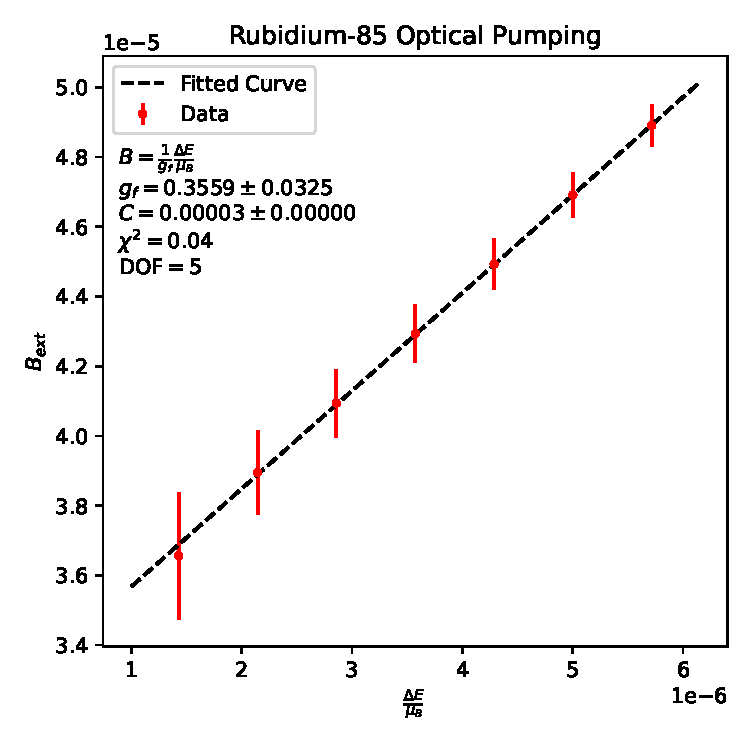
\includegraphics[width=0.75\textwidth]{experiment4/figures/rb85.pdf}
    \caption{Zeeman equation fit for Rubidium-85 isotope. The fitted Landé g-factor is within a margin of error of expected values $g_f = \frac{1}{3}$}
    \label{fig:rb85}
\end{figure}

\begin{figure}[!h]
    \centering
    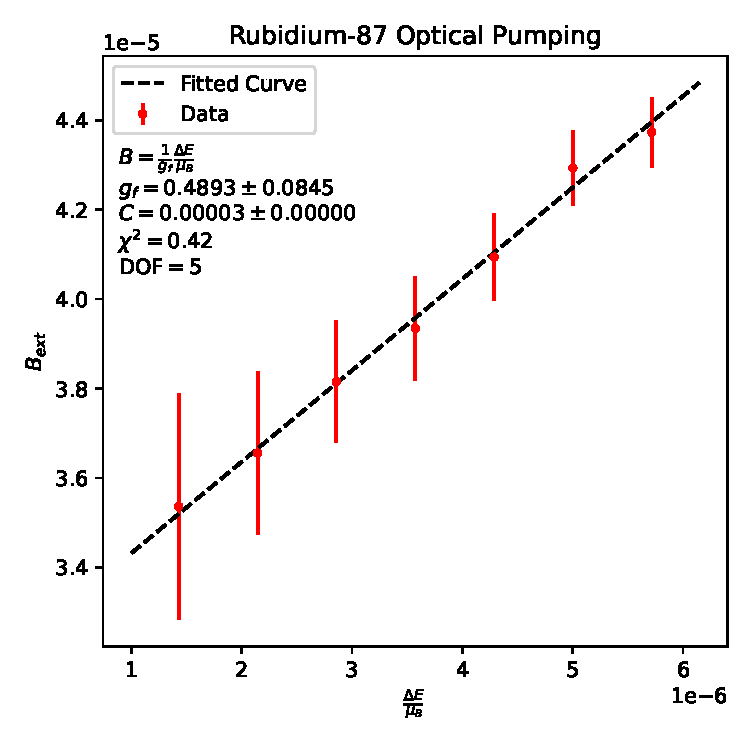
\includegraphics[width=0.75\textwidth]{experiment4/figures/rb87.pdf}
    \caption{Zeeman equation fit for Rubidium-87 isotope. The fitted Landé g-factor is within a margin of error of expected values $g_f = \frac{1}{2}$}
    \label{fig:rb87}
\end{figure}

Evidently, the fits we produced are very good. Visually, they model the data very well, and we achieve reasonble uncertainty on our fit parameters. The reduced chi-square is $\bar{\chi}^2=0.008$ for Rb-85 $\bar{\chi}^2=0.084$ for Rb-87, which indicate overfitting or poor error modeling. We hypothesize that we significantly overestimated our uncertainties, thus producing these small values. 

\subsection{A discussion on the fit intercept}

Where did the intercept $C$ come from? We observed that, without this intercept term, we are unable to obtain a satisfactory fit. Our hypothesis is that $C$ corresponds to the ambient magnetic field $B_a$ of the room we were unable to remove. Indeed, we can write:
\begin{align*}
    \Delta E &= \mu_B g_f (B + B_{a}) \\
    \Rightarrow B &= \frac{1}{g_f} \frac{\Delta E}{\mu_B} - B_a
\end{align*}
We can check that both fits estimate consistent values for $C$ or $-B_a$. The Rb-85 fit gives $C = 0.000033 \pm 0.0000012$ and the Rb-87 fit gives $C = 0.000032 \pm 0.0000016$, which are within margins of error of each other. This lend creedence to our hypothesis, as ostensibly the ambient field should be constant. 

\section{The strong field Zeeman effect} \label{sec:strong}

Now we briefly explore the strong field Zeeman effect. Using an external power source, we apply a large magnetic field to the rubidium and study the further splitting of the depumping dips. Figures \ref{fig:rb85strong} and \ref{fig:rb87strong} show these individual dips for Rb-85 and Rb-87 respectively. 

\begin{figure}[!h]
    \centering
    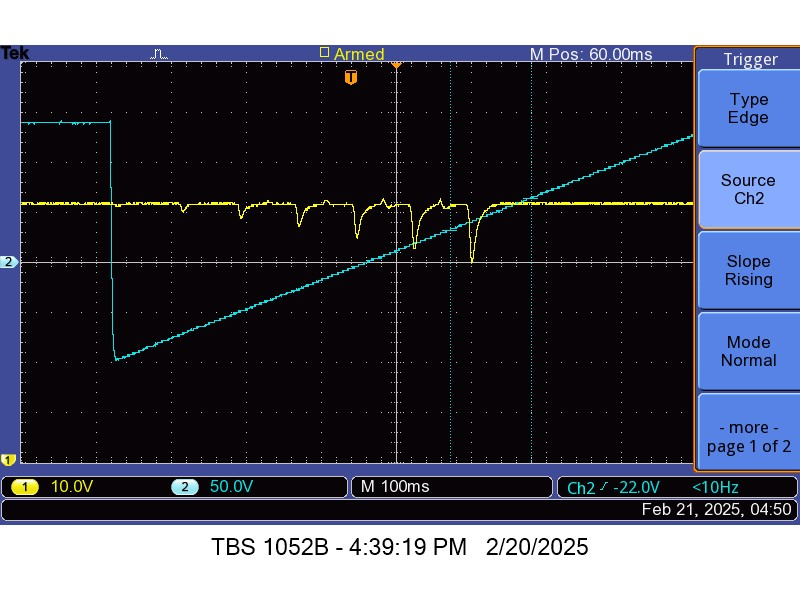
\includegraphics[width=0.75\textwidth]{experiment4/figures/rb85_strong.jpg}
    \caption{Strong field Zeeman splitting of Rb-85 depumping dip into 6 dips. The RF frequency used was 5.690 MHz and the horizontal coil current supplied was 1.41 amps.}
    \label{fig:rb85strong}
\end{figure}

\begin{figure}[!h]
    \centering
    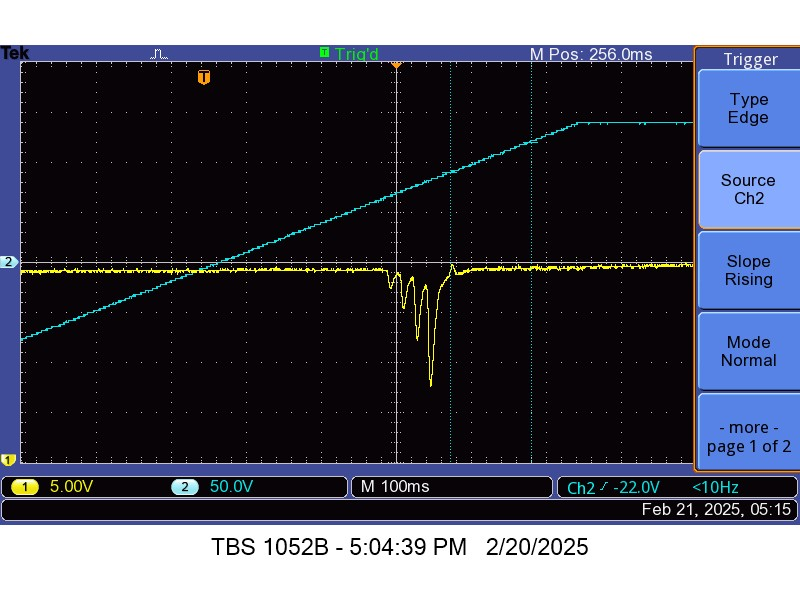
\includegraphics[width=0.75\textwidth]{experiment4/figures/rb87_strong.jpg}
    \caption{Strong field Zeeman splitting of Rb-87 depumping dip into 4 dips. The RF frequency used was 5.000 MHz and the horizontal coil current supplied was 0.84 amps.}
    \label{fig:rb87strong}
\end{figure}

From these oscilloscope traces, we can deduce the nuclear spin quantum number $I$. Let the number of dips be $d$. Each dip corresponds to a transition between Zeeman levels, so there must be $d + 1$ Zeeman levels. But the number of Zeeman levels is $2F + 1$ so $d = 2F$. We then get $F = 3$ for Rb-85 and $F=2$ for Rb-87. We know $J=\frac{1}{2}$ for both isotopes, so using $I = F - J$ we arrive at $I = \frac{5}{2}$ for Rb-85 and $I = \frac{3}{2}$ for Rb-87. 

\section{Conclusion}

Now we can compute the theoretical Landé g-factors for Rb-85 and Rb-87 and compare with our estimates from \ref{sec:weak}. The Landé g-factor is given in terms of quantum numbers by:
\begin{equation}
    g_f = g_j \frac{F(F+1) + J(J+1) - I(I+1)}{2F(F+1)}
\end{equation}
where
\begin{equation}
    g_j = 1 - \frac{J(J+1) + S(S+1) - L(L+1)}{2J(J+1)}
\end{equation}
Now, for both Rb-85 and Rb-87, $J=S=\frac{1}{2}$ and $L=J-S=0$, so
\begin{equation}
    g_j = 1 + \frac{\frac{1}{2}(\frac{1}{2}+1) + \frac{1}{2}(\frac{1}{2}+1)}{2 \cdot \frac{1}{2}(\frac{1}{2}+1)} = 2
\end{equation}
Then for Rb-85:
\begin{equation}
    g_f = 2 \cdot \frac{3(3+1) + \frac{1}{2}(\frac{1}{2}+1) - \frac{5}{2}(\frac{5}{2}+1)}{2 \cdot 3(3+1)} = \frac{1}{3}
\end{equation}
And for Rb-87:
\begin{equation}
    g_f = 2 \cdot \frac{2(2+1) + \frac{1}{2}(\frac{1}{2}+1) - \frac{3}{2}(\frac{3}{2}+1)}{2 \cdot 2(2+1)} = \frac{1}{2}
\end{equation}
Thus, our fitted values of $g_f = 0.356 \pm 0.032$ and $g_f = 0.489 \pm 0.084$ for Rb-85 and Rb-87, respectively, are well within a margin of error of the theoretical values, and we can claim agreement. 

Overall, we have observed good conformance to theory in this lab. All our theoretical predictions have been confirmed within uncertainty bounds by our empirical estimates. However, we have observed some subpar fitting statistics, such as reduced chi-squared values that are too high or too low. In the future, it would be wise to be more thorough with data collection—namely taking more samples—as well as uncertainty estimation. In particular, here we saw some consequences of overestimating uncertainty as reflected in poor reduced chi-square values. 

\end{document}
